\documentclass[12pt, oneside]{article}   	% use "amsart" instead of "article" for AMSLaTeX format
\usepackage{geometry}                		% See geometry.pdf to learn the layout options. There are lots.
\geometry{letterpaper}                   		% ... or a4paper or a5paper or ... 

\usepackage{graphicx}				% Use pdf, png, jpg, or eps§ with pdflatex; use eps in DVI mode
								% TeX will automatically convert eps --> pdf in pdflatex		
\usepackage{amssymb}

\usepackage{xcolor}

\usepackage{fullpage}

\title{Implementing a Neural Net for Stock Forecasting}
\author{Helen Mehreteab and Anusha Murali}
%\date{}							% Activate to display a given date or no date

\begin{document}
\maketitle
\section{Description}

Predicting the price of a company stock is one of the most difficult tasks, even for experienced traders. The future value of a stock is dependent on numerous factors such as the company's financial health , the historical stock prices, analyst repots, and the general market volatility.  In this project, we use the historical stock prices of a company to predict its future stock prices. Using three popular machine learning algorithms, namely linear regression, Prophet and Long Short Term Memory (LSTM) algorithm, and elementary data manipulations on widely available CSV data for publicly traded companies,  we demonstrate that one could predict stock prices with a high degree of accuracy.

Our program, called {\tt cs50stock} was written in Python, and can be run from any platform that has Python version 3.7.5 or higher.

\section{Getting Started}
The following instructions outline how to get the project up and running on a local machine for both development and testing purposes.

\subsection{Prerequisites}

Our project was developed using Python 3.7.5 on Mac OSX. The source code is entirely contained in a single Python file called {\tt cs50stock.py}.  The following Python libraries are necessary to run {\tt cs50stock}:

\subsubsection{Mandatory Python Packages}
Our project has absolute dependency on the following Python packages.
\begin{enumerate}
\item {\tt pandas}
\item {\tt numpy}
\item {\tt matplotlib}
\item {\tt sklearn}
\item {\tt keras}
\item {\tt fbprophet}
\item {\tt fastai} \textcolor{red}{It is important to have version 0.7.0 of {\tt fastai} installed as the most recent version does not support the {\tt structured} module}. It took as more than three hours to figure out that the latest version of {\tt fastai} has many modules renamed from the earlier versions.
\item {\tt torch} \textcolor{red}{It is important to have version 0.1.2 of {\tt torch} installed on the system as {\tt fastai} is dependent on it.}
\end{enumerate}

\subsubsection{Supplementary Python Packages}
The following packages are not mandatory to successfully run our program. The absence of the following packages will result in warning messages, but will not prevent one from running the code to successful completion. 
\begin{enumerate}
\item {\tt sys}
\item {\tt warnings}
\item {\tt platform}
\item {\tt subprocess}
\item {\tt time}
\end{enumerate}

\subsubsection{Data Files}

The program expects one or more CSV files in the directory where {\tt cs50stock.py} is found. These files contain the historical stock data in CSV format. We have made the following files available for testing purposes: {\tt IBM.csv, MSFT.csv, ORCL.csv, FB.csv, AMZN.csv, GOOG.csv, NFLX.csv, } and {\tt AAPL.csv}. 
More CSV files can be downloaded from {\tt finance.yahoo.com}.

\section{Running {\tt cs50stock}}

Please note that our program requires Python version 3.0. The program can be started by running \\

\centerline{\tt \$ python3 cs50stock.py} 

\vspace{0.2in}
\noindent
from the terminal on a Mac. \\


\noindent
The program can also be run from {\tt IDLE}, which is one of the popular Python editors. However, we have noticed that the Python shell spawned from {\tt IDLE} may not always properly format tabular outputs generated by the {\tt PrettyTable} Python package. Therefore, we strongly recommend that you run our program from a terminal window on a Mac.\\

\noindent
When the program is launched, the following screen first appears allowing the user to select from a set of eight sample stock symbols.\\

\centerline{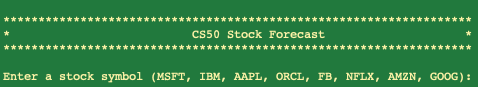
\includegraphics[width=5.5in]{1.png}}

\vspace{0.2in}
\noindent
Selecting one of the above symbols takes the user to the following menu:\\

\centerline{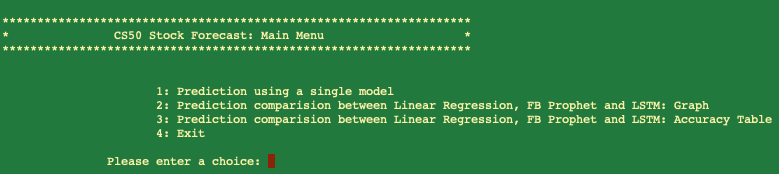
\includegraphics[width=6.5in]{2.png}}

\vspace*{0.2in}

\noindent
As seen from the above menu, the program has three major features:

\begin{enumerate}
\item Stock forecasting using a specific machine learning model (i.e: Linear regression, FB Prophet, and LSTM).
\item Graphical comparison of the three machine learning models (i.e: Linear regression, FB Prophet, and LSTM).
\item Error rates of the three machine learning models (i.e: Linear regression, FB Prophet, and LSTM).
\end{enumerate}

\noindent
Selecting Option \#1 from the Main menu presents the user with the following set of options:\\


\centerline{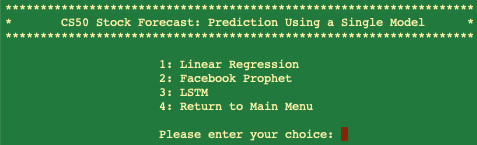
\includegraphics[width=6in]{3.png}}

\vspace*{0.2in}
\noindent
As can be seen from the above menu,  the user can now choose one of the following Machine Learning algorithms for stock forecasting:
\begin{enumerate}
\item Linear Regression,
\item Facebook Prophet or 
\item LSTM
\end{enumerate}
For example, selecting {\tt IBM.csv} and {\tt Linear Regression} generates the following plot.  The green line on the right corresponds to the test data (which is nearly 20\% of the historical data), and closely tracks the actual test data presented in orange. Therefore, the user can see that the {\tt Linear Regression} model is fairly accurate enough to predict the stock values.\\

\centerline{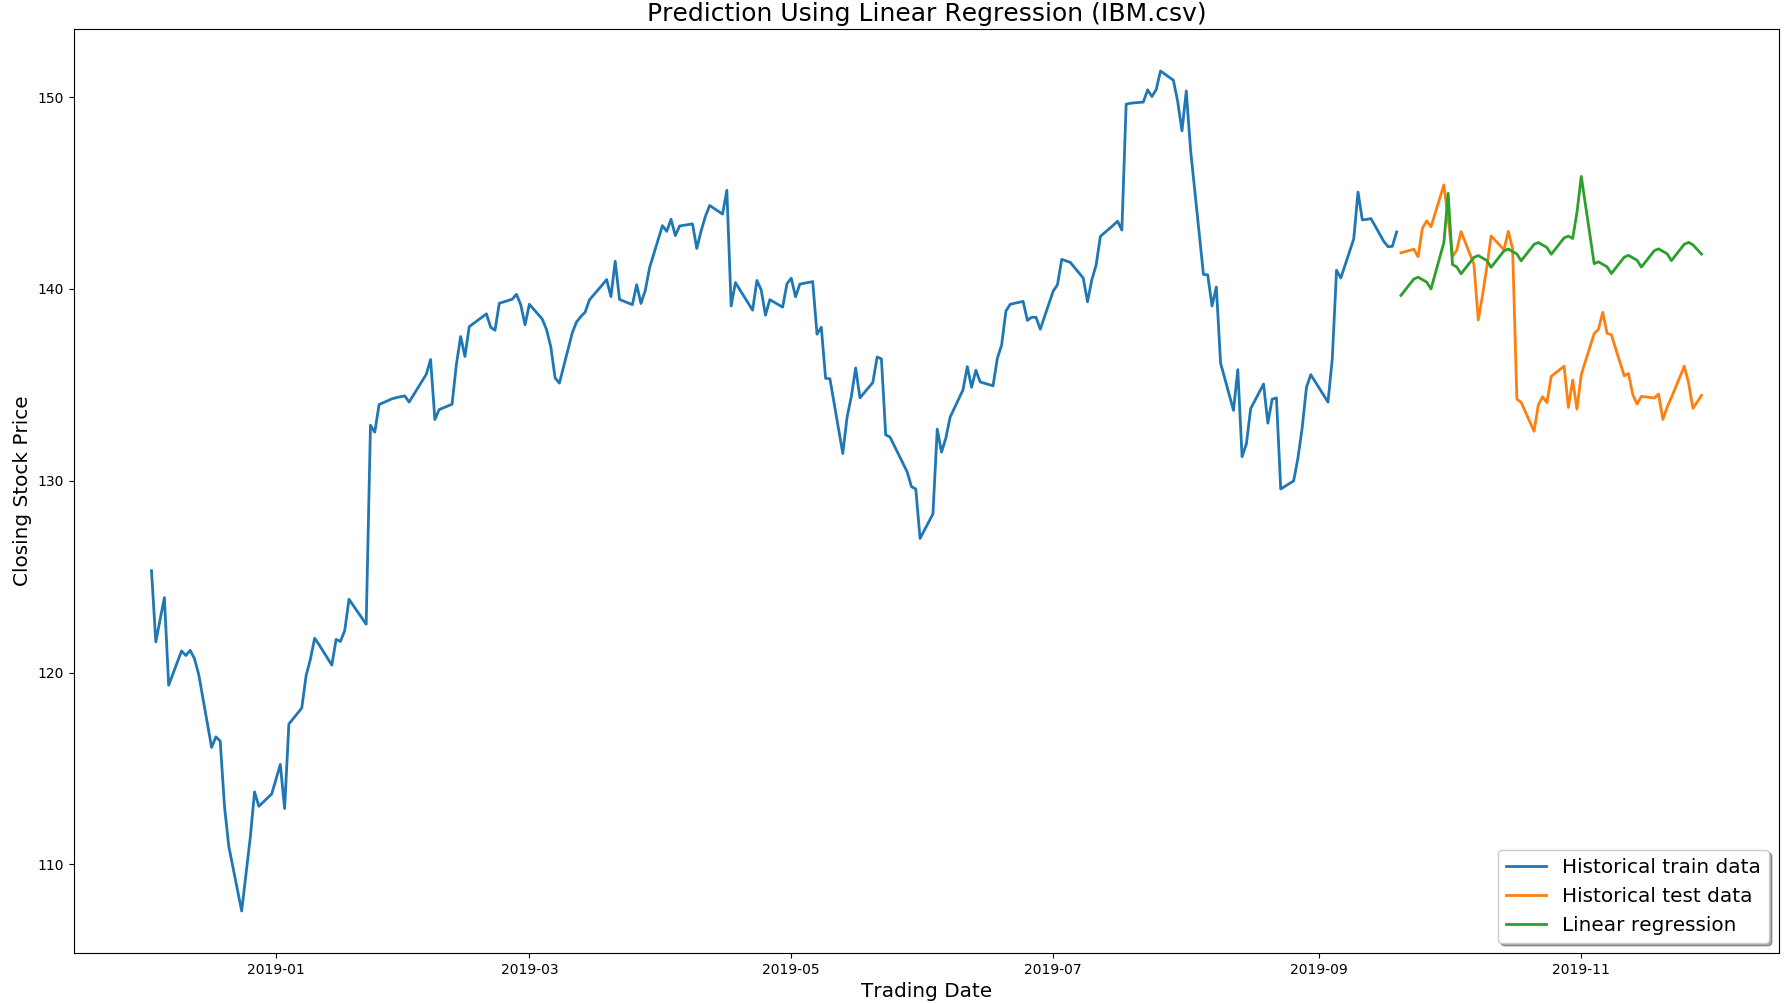
\includegraphics[width=6in]{LR.png}}

\noindent
Selecting Option \#2 from the Main menu generates a combined plot from all three algorithms, which allows the user to compare their performances for various data inputs. For example,  for {\tt IBM.csv}, we obtain the following plot:

\centerline{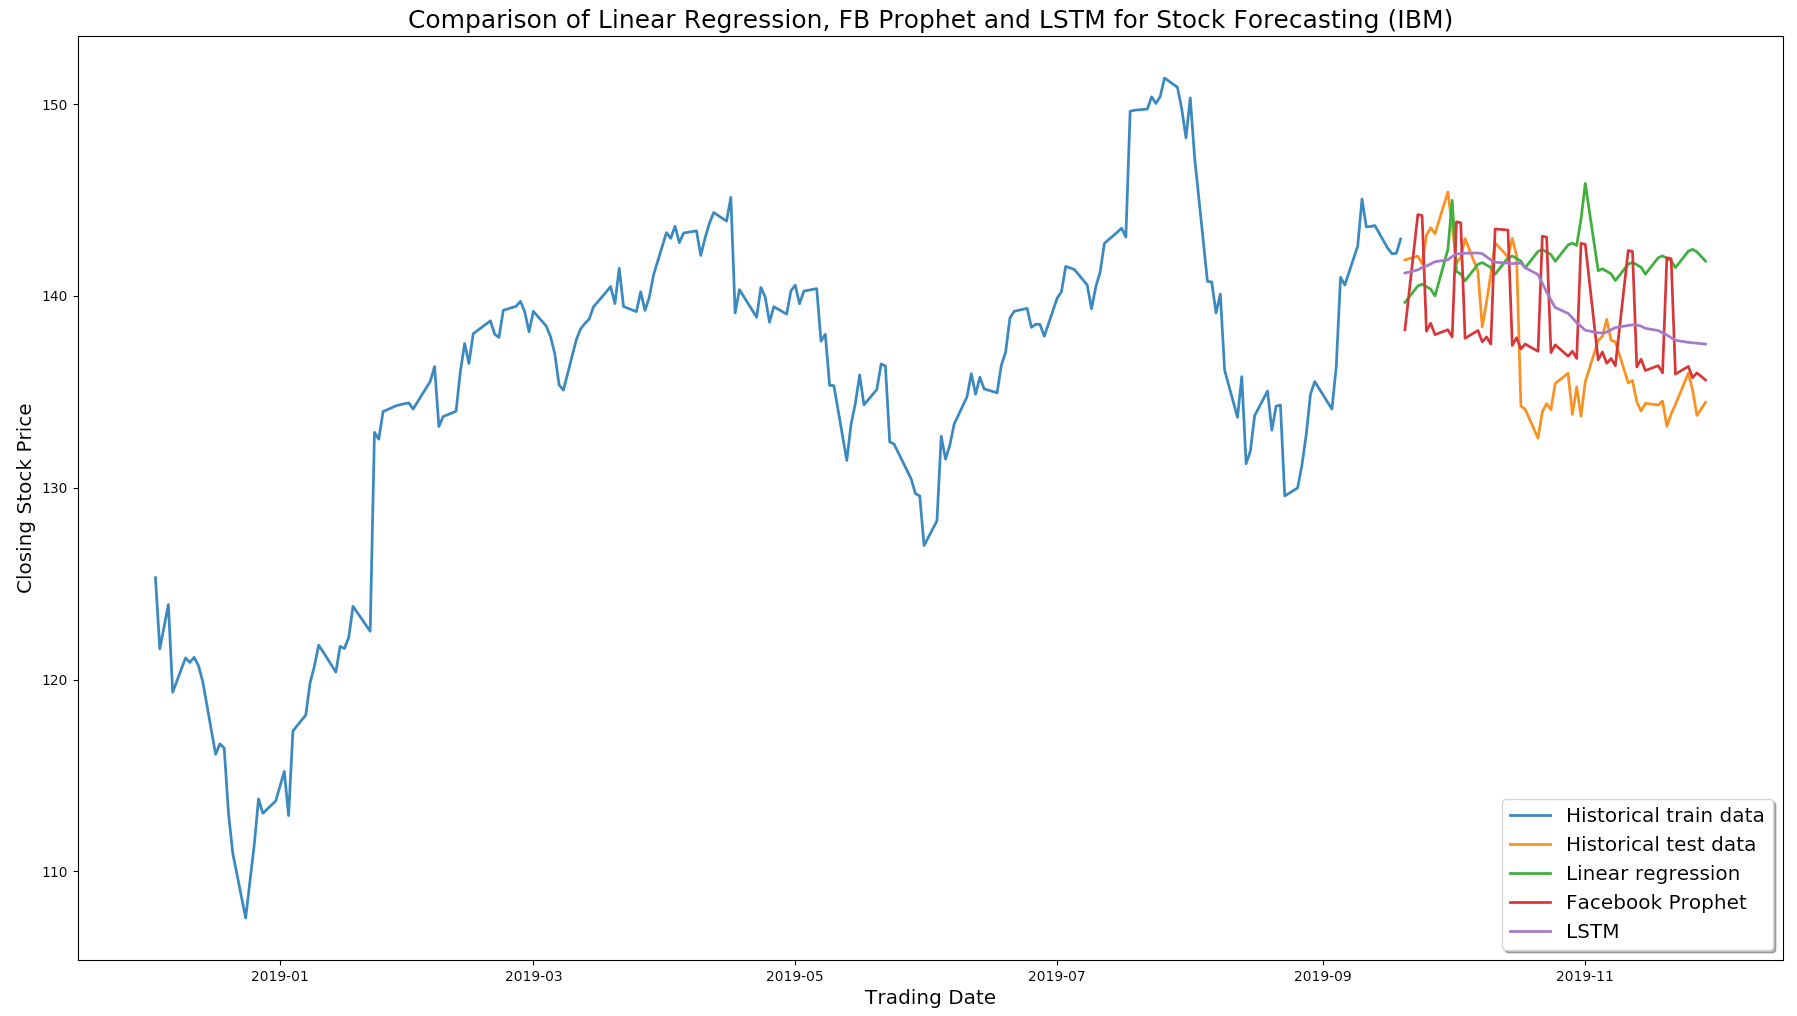
\includegraphics[width=6in]{ALL.png}}

\vspace*{0.2in}
\noindent
Finally, selecting Option \#3 from the Main menu generates the following tabular output, which shows the error rate from the three algorithms:\\

\centerline{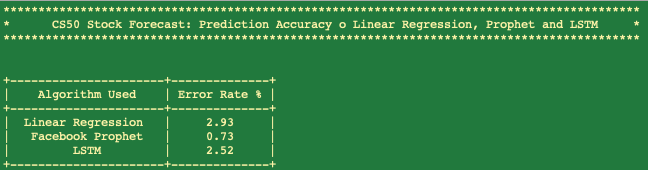
\includegraphics[width=6.5in]{4.png}}


\section{Authors}
\begin{itemize}
\item Helen Mehreteab 
\item Anusha Murali
\end{itemize}


\section{Acknowledgments}

\begin{enumerate}
\item Gad, Ahmed., From $y$-$x$ to building a complete artificial neural network
\item Koehrsen, Will., Stock Analysis in Python
\item Numerous ML videos from {\tt 3blue1brown.com}
\end{enumerate}


\end{document}  